Kamera termal digunakan sebagai sensor pelengkap untuk mengatasi keterbatasan LiDAR dua dimensi dalam mendeteksi obstacle berprofil rendah yang berada di luar bidang pindai horizontal. Berbeda dengan LiDAR yang mengukur jarak berdasarkan pantulan sinar laser, kamera termal menghasilkan citra yang merepresentasikan distribusi energi inframerah pada lingkungan. Karakteristik tersebut memungkinkan objek yang memiliki perbedaan temperatur terhadap lingkungan sekitarnya tetap dapat dikenali meskipun tidak terdeteksi oleh sensor laser (\cite{Castro2016,Choi2023}).

Pada penelitian ini, data termal tidak digunakan secara langsung sebagai masukan navigasi. Citra termal terlebih dahulu diproses melalui beberapa tahapan yang meliputi akuisisi citra, segmentasi semantik, ekstraksi fitur traversability, serta identifikasi area blind-spot. Hasil pemrosesan tersebut digunakan untuk menghasilkan representasi lingkungan yang dapat dimanfaatkan oleh sistem navigasi.

\subsection{Akuisisi Citra Termal}

Kamera termal dimodelkan menggunakan \textit{plugin} Gazebo \texttt{libgazebo\_ros\_thermal\_c\-amera} dari paket \texttt{hector\_gazebo\_thermal\_camera}. Sensor ini menghasilkan citra termal berformat \texttt{L8} (\textit{8-bit grayscale}) dengan resolusi $640 \times 480$ piksel pada frekuensi 10 Hz.

Data citra dipublikasikan melalui topik:

\begin{center}
\texttt{/thermal/thermal\_camera/image\_raw}
\end{center}

Dalam representasi ini, nilai piksel yang lebih tinggi menunjukkan temperatur relatif yang lebih tinggi dibandingkan lingkungan sekitarnya. Dengan demikian, manusia, hewan, dan objek yang memancarkan panas cenderung muncul sebagai area yang lebih terang dibandingkan lantai atau dinding.

\subsection{Segmentasi Semantik Citra Termal}

Tahap pertama pemrosesan dilakukan oleh node \texttt{semantic\_thermal.py}. Tujuan utama tahap ini adalah mengubah citra termal mentah menjadi representasi semantik yang membedakan area obstacle dan area yang dapat dilalui robot.

Sebelum proses segmentasi dilakukan, citra terlebih dahulu mengalami koreksi orientasi dan pemotongan \textit{region of interest} (ROI). ROI difokuskan pada area lantai di depan robot sehingga proses analisis tidak terpengaruh oleh objek yang berada jauh dari jalur navigasi.

Setelah ROI diperoleh, citra mengalami proses peningkatan kualitas menggunakan kombinasi \textit{Gaussian blur} dan \textit{image sharpening}. Proses ini bertujuan memperjelas batas termal antara obstacle dan lingkungan sekitarnya sehingga segmentasi menjadi lebih stabil.

Segmentasi dilakukan menggunakan metode berbasis ambang intensitas (\textit{threshold-based segmentation}). Pendekatan ini dipilih karena citra termal yang dihasilkan simulator memiliki distribusi intensitas yang relatif stabil dan tidak memerlukan proses pelatihan model seperti pada metode berbasis \textit{deep learning} (\cite{Castro2016}).

Berdasarkan nilai intensitas piksel, citra dibagi menjadi tiga kelas utama sebagaimana ditunjukkan pada Tabel~\ref{tab:kelas_segmentasi_termal}.

\begin{table}[H]
\centering
\caption{Kelas segmentasi termal berdasarkan rentang intensitas piksel}
\label{tab:kelas_segmentasi_termal}
\begin{tabular}{llll}
\toprule
\textbf{Kelas} &
\textbf{Rentang Intensitas} &
\textbf{Representasi} &
\textbf{Visualisasi} \\
\midrule
Lantai dapat dilalui &
$[45,72]$ &
Area navigasi &
Hijau \\

Obstacle termal &
$[73,255]$ &
Manusia atau hewan &
Merah \\

Objek dingin &
$[0,44]$ &
Dinding dan objek statis &
Hitam \\
\bottomrule
\end{tabular}
\end{table}

Untuk meningkatkan kualitas segmentasi, hasil klasifikasi kemudian diproses menggunakan operasi morfologi. Operasi \textit{closing} digunakan untuk menghubungkan area lantai yang terputus akibat noise, sedangkan operasi \textit{opening} digunakan untuk menghilangkan blob termal berukuran kecil yang tidak merepresentasikan obstacle nyata.

Hasil akhir tahap ini dipublikasikan sebagai citra semantik melalui topik \texttt{/semantic\_m\-ask}.

\begin{figure}[H]
\centering
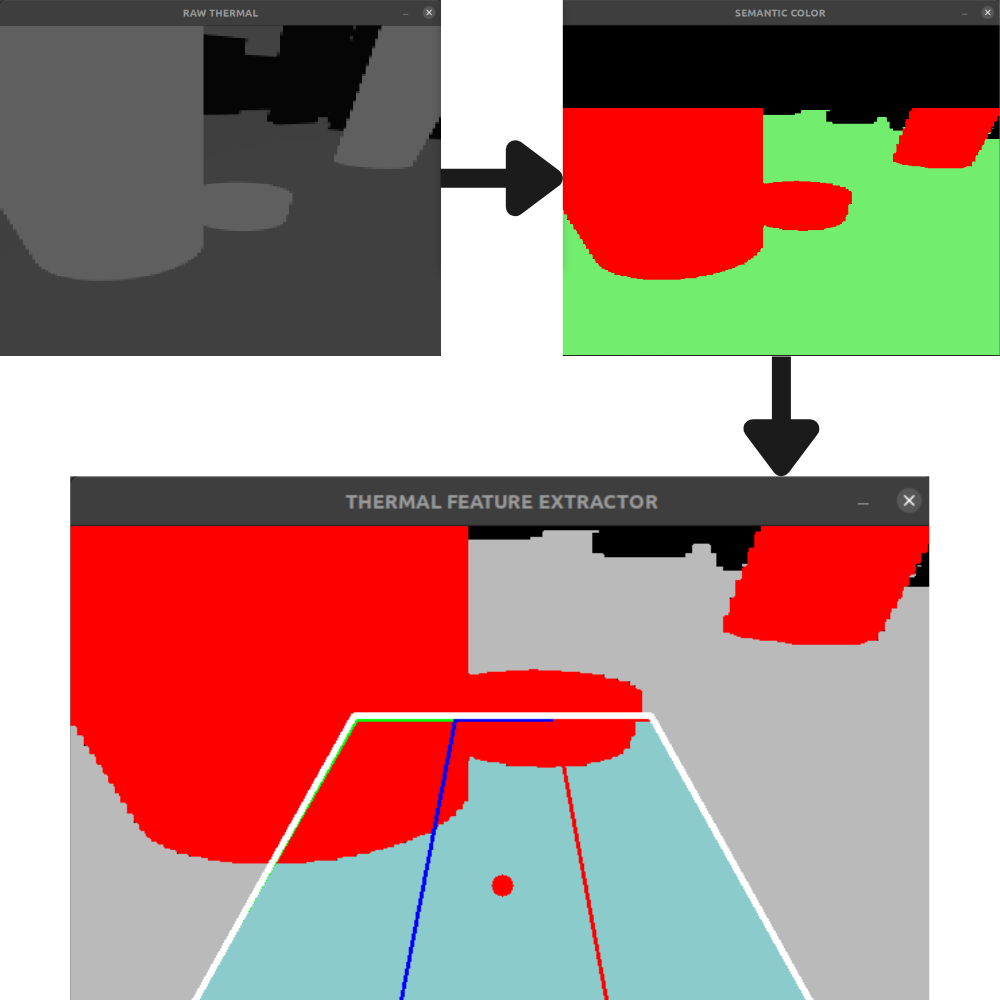
\includegraphics[width=0.5\textwidth]{gambar/3.5_segmentasi_termal.png}
\caption{Contoh hasil segmentasi semantik pada citra termal.}
\label{fig:segmentasi_termal}
\end{figure}

\subsection{Ekstraksi Fitur Traversability}

Setelah proses segmentasi selesai, citra semantik diproses oleh node \texttt{thermal\_feature\-\_extractor.py}. Tahap ini bertujuan mengekstraksi informasi lingkungan yang lebih ringkas dan mudah digunakan oleh sistem navigasi.

Untuk memperoleh informasi yang relevan terhadap pergerakan robot, diterapkan ROI berbentuk trapesium yang merepresentasikan area pengamatan di depan robot. Bentuk trapesium dipilih untuk menyesuaikan perspektif kamera sehingga area yang lebih dekat terhadap robot memiliki bobot pengamatan yang lebih besar.

Berdasarkan ROI tersebut, sistem menghitung skor traversability termal yang merepresentasikan tingkat keterlaluan area di depan robot. Nilai traversability dinyatakan dalam rentang $[0,1]$, dengan nilai mendekati satu menunjukkan area yang relatif bebas obstacle, sedangkan nilai mendekati nol menunjukkan area yang didominasi obstacle termal.

Secara umum, skor traversability dihitung berdasarkan rasio antara area bebas dan area obstacle yang berada di dalam ROI. Nilai ini digunakan sebagai indikator kondisi lingkungan yang nantinya akan digabungkan dengan informasi LiDAR pada proses fusi sensor.

Selain traversability, sistem juga menghitung lebar koridor bebas (\textit{corridor width}) dan posisi tengah koridor (\textit{center path}). Kedua parameter tersebut digunakan untuk menggambarkan distribusi ruang bebas yang tersedia di depan robot.

\subsection{Analisis Zona Navigasi}

Untuk memperoleh informasi spasial yang lebih rinci, area ROI dibagi menjadi tiga zona navigasi, yaitu zona kiri, zona tengah, dan zona kanan. Pembagian ini memungkinkan sistem mengidentifikasi distribusi obstacle secara lateral tanpa harus melakukan analisis citra secara penuh pada setiap siklus pemrosesan.

Pada masing-masing zona dihitung rasio area bebas terhadap total area zona. Nilai rasio tersebut digunakan untuk menunjukkan tingkat keterlaluan setiap sisi jalur navigasi.

Sebagai contoh, apabila nilai zona kiri lebih rendah dibandingkan zona kanan, maka dapat diinterpretasikan bahwa obstacle lebih dominan berada pada sisi kiri robot. Informasi ini berguna untuk membantu sistem menentukan arah penghindaran obstacle yang lebih aman (\cite{Sevastopoulos2022}).

\subsection{Deteksi Area Blind-Spot}

Selain digunakan untuk menghitung traversability, citra termal juga dimanfaatkan untuk mengidentifikasi obstacle yang tidak terdeteksi oleh LiDAR akibat keterbatasan bidang pindai horizontal. Obstacle yang berada pada area blind-spot akan tetap muncul pada citra termal selama memiliki perbedaan temperatur yang cukup terhadap lingkungan sekitarnya.

Untuk tujuan tersebut, node \texttt{semantic\_thermal.py} menghasilkan masker obstacle termal yang dipublikasikan melalui topik:

\begin{center}
\texttt{/thermal\_obstacle\_mask}
\end{center}

Masker ini berisi representasi biner obstacle termal yang telah dipisahkan dari area lantai dan objek latar belakang. Informasi tersebut menjadi dasar untuk membangun representasi obstacle blind-spot pada tahap berikutnya.

Pada tahap ini, informasi termal masih berada dalam domain citra dan belum digunakan secara langsung oleh sistem navigasi. Integrasi dengan data LiDAR dilakukan melalui proses pembentukan \textit{Virtual LaserScan} dan fusi traversability yang akan dijelaskan pada Subbab~\ref{sec:fusi_traversability}.